\section{梯度下降解一元线性回归}
\label{sec:chapter1}

\subsection{一元线性回归}

给定如下数据集：
\[
\left\{\left(x^{(i)},y^{(i)}\right),\;i=1,2,\cdots,m\right\}
\]
其中，$m$ 表示样本数量，$x^{(i)}$ 与 $y^{(i)}$ 分别表示第 $i$ 个样本的输入和对应的观测值。一元线性回归的目标是使用线性函数 $y=\theta_1x+\theta_0$ 对这些数据进行拟合。虽然该问题可以直接通过最小二乘法求得解析解，但本节以它为例介绍如何使用梯度下降法迭代求解。


\subsection{梯度下降法}

梯度下降法是一种常用的迭代优化算法。对于代价函数 $J(\theta_0,\theta_1)$，其基本思路是从一个初始参数点出发，沿当前点负梯度所指示的下降方向移动一小步，并反复执行这一过程，从而逐步减小代价函数的取值。若代价函数满足适当的凸性与光滑性条件，该过程可以收敛到其全局最小值；在更一般的情况下，梯度下降法通常用于寻找局部极小值或驻点。

函数 $J$ 关于参数 $\theta_0$ 和 $\theta_1$ 的梯度定义为：
\[
\text{grad }J=\left\{\frac{\partial J}{\partial \theta_0},\frac{\partial J}{\partial \theta_1}\right\}
\]
因此，可以按照下式不断更新参数：
\[
\theta_j:=\theta_j-\alpha\cdot\frac{\partial J}{\partial\theta_j},\quad j=0,1
\]
其中，$\alpha$ 表示每次更新的步长，通常称为\textbf{学习率}。需要注意的是，在一次迭代中，$\theta_0$ 和 $\theta_1$ 应当依据更新前的参数值同步计算并更新。

学习率的选取会直接影响算法的收敛速度和稳定性。学习率过小时，每次参数更新的幅度有限，因而收敛过程可能较慢；学习率过大时，参数则可能越过极小值附近的区域并反复振荡，甚至导致算法无法收敛。


\subsection{梯度下降解一元线性回归}

为了衡量模型预测值与真实观测值之间的差异，定义代价函数为：
\[
J(\theta_0,\theta_1)=\frac{1}{2m}\sum_{i=1}^m\left(\theta_1x^{(i)}+\theta_0-y^{(i)}\right)^2
\]
该函数是所有样本预测值与真实值的均方误差。

对代价函数分别关于 $\theta_0$ 和 $\theta_1$ 求偏导，可得：
\[
\text{grad }J=\left\{\frac{\partial J}{\partial \theta_0},\frac{\partial J}{\partial \theta_1}\right\}=\left\{\frac{1}{m}\sum_{i=1}^m\left(\theta_1x^{(i)}+\theta_0-y^{(i)}\right),\frac{1}{m}\sum_{i=1}^mx^{(i)}\left(\theta_1x^{(i)}+\theta_0-y^{(i)}\right)\right\}
\]
将上述两个偏导数代入参数更新公式，即可在每次迭代中沿负梯度方向调整 $\theta_0$ 和 $\theta_1$.


\subsection{代码实现}
\paragraph{C++ 实现}

对于该问题，可以预先计算样本中若干与参数无关的求和项，使每次梯度更新的时间复杂度降为 $O(1)$.

\begin{lstlisting}[language=C++]
#include<bits/stdc++.h>

using namespace std;

const double eps = 1e-8;
const double alpha = 0.01;

int m;
double sumx, sumy, sumxy, sumx2;
double th0, th1;

int main(){
	freopen("ex1data1.txt", "r", stdin);
	double x, y;
	while(scanf("%lf,%lf", &x, &y) != EOF)
		m++, sumx += x, sumy += y, sumx2 += x * x, sumxy += x * y;
	th0 = th1 = 0;
	while(1){
		double nth0, nth1;
		nth0 = th0 - alpha * 1.0 / m * (th1 * sumx - sumy + m * th0);
		nth1 = th1 - alpha * 1.0 / m * (th1 * sumx2 - sumxy + sumx * th0);
		if(fabs(th0 - nth0) < eps && fabs(th1 - nth1) < eps)	break;
		th0 = nth0, th1 = nth1;
	}
	printf("%f %f\n", th0, th1);
	return 0;
}
\end{lstlisting}

程序得到的结果为：$\theta_0=-3.895775,\,\theta_1=1.193033$.

若将 $\alpha$ 设为 $0.1$，上述程序将无法获得收敛结果。这是因为学习率过大，参数更新可能在极小值附近反复跨越，导致代价函数无法稳定下降。除直接减小 $\alpha$ 之外，还可以让程序根据迭代过程自适应地调整学习率。具体地，当学习率取值合理时，代价函数通常应当随迭代逐步减小。因此，如果一次参数更新后代价函数反而增大，就可以将其视为当前学习率过大的信号，并相应减小 $\alpha$。基于这一思路，可以得到如下实现：

\begin{lstlisting}[language=C++]
#include<bits/stdc++.h>

using namespace std;

const int N = 105;
const double eps = 1e-8;
double alpha = 100;

int m;
double x[N], y[N];
double th0, th1;

inline double gradJ(int k){
	double res = 0;
	for(int i = 1; i <= m; i++)
		res += (th1 * x[i] + th0 - y[i]) * (k == 1 ? x[i] : 1);
	return res / m;
}

inline double calc(){
	double res = 0;
	for(int i = 1; i <= m; i++)
		res += (th1 * x[i] + th0 - y[i]) * (th1 * x[i] + th0 - y[i]);
	return res / m / 2;
}

int main(){
	freopen("ex1data1.txt", "r", stdin);
	while(scanf("%lf,%lf", &x[0], &y[0]) != EOF)
		m++, x[m] = x[0], y[m] = y[0];
	th0 = th1 = 0;
	double preJ = 1e9, J = 0;
	while(1){
		double nth0, nth1;
		nth0 = th0 - alpha * gradJ(0);
		nth1 = th1 - alpha * gradJ(1);
		if(fabs(th0 - nth0) < eps && fabs(th1 - nth1) < eps)	break;
		th0 = nth0, th1 = nth1;
		J = calc();
		if(J > preJ)	alpha /= 5;
		preJ = J;
	}
	printf("%f\n%f %f\n", alpha, th0, th1);
	return 0;
}
\end{lstlisting}

最终得到的结果为：$\alpha=0.0064,\,\theta_0=-3.895772,\,\theta_1=1.193033$.


\paragraph{Python 实现}

Python 拥有较为完善的可视化工具，常用于机器学习算法的实现和实验分析。
如下是学习率设置为 0.01 的 Python 代码：

\begin{lstlisting}[language=Python]
import numpy as np
import matplotlib.pyplot as plt

X = []
Y = []
m = 0
alpha = 0.01
eps = 1e-8
th0, th1 = 0, 0

def gradJ(k):
	res = 0
	for x, y in zip(X, Y):
		res += (th1 * x + th0 - y) * (x if k == 1 else 1)
	return res / m

def calc():
	res = 0
	for x, y in zip(X, Y):
		res += (th1 * x + th0 - y) * (th1 * x + th0 - y)
	return res / 2 / m

with open("ex1data1.txt", "r") as infile:
	data = infile.readlines()
	for line in data:
		x, y = line.split(',')
		X.append(float(x))
		Y.append(float(y))
		m += 1


while 1:
	nth0 = th0 - alpha * gradJ(0)
	nth1 = th1 - alpha * gradJ(1)
	if abs(th0 - nth0) < eps and abs(th1 - nth1) < eps:
		break
	th0 = nth0
	th1 = nth1
print(th0, th1)
plt.scatter(X, Y)
plt.plot([min(X), max(X)], [th0+min(X)*th1, th0+max(X)*th1], c="magenta")
plt.show()
\end{lstlisting}

程序得到的结果为：$\theta_0=-3.895775,\,\theta_1=1.193033$，原始数据及拟合效果如下图所示：

\begin{figure}[H]
    \centering
    \begin{minipage}{0.4\linewidth}
        \centering
        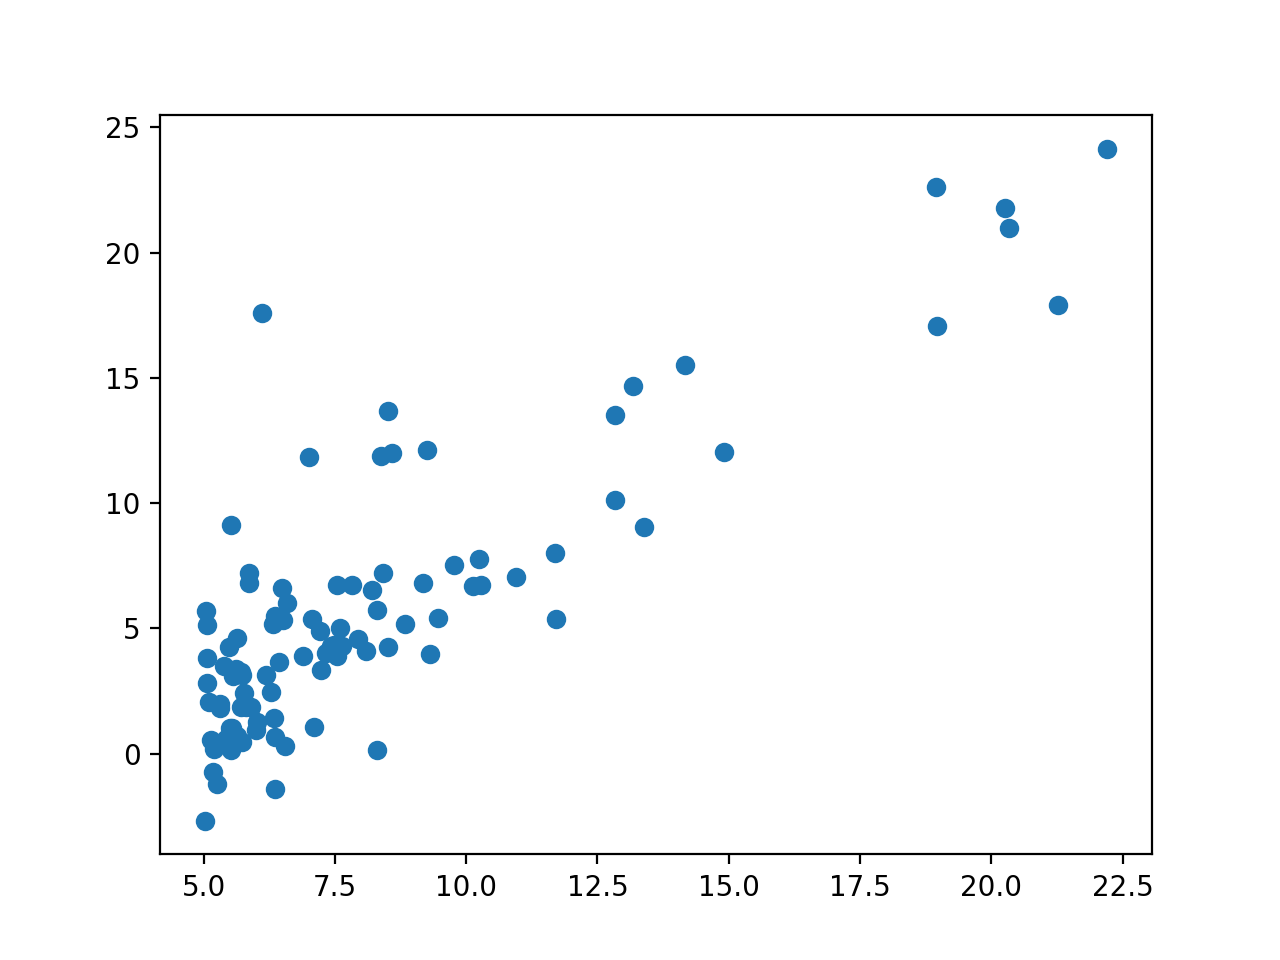
\includegraphics[width=\linewidth]{figs/Chap_1_Figure_1.png}
    \end{minipage}
    \begin{minipage}{0.4\linewidth}
        \centering
        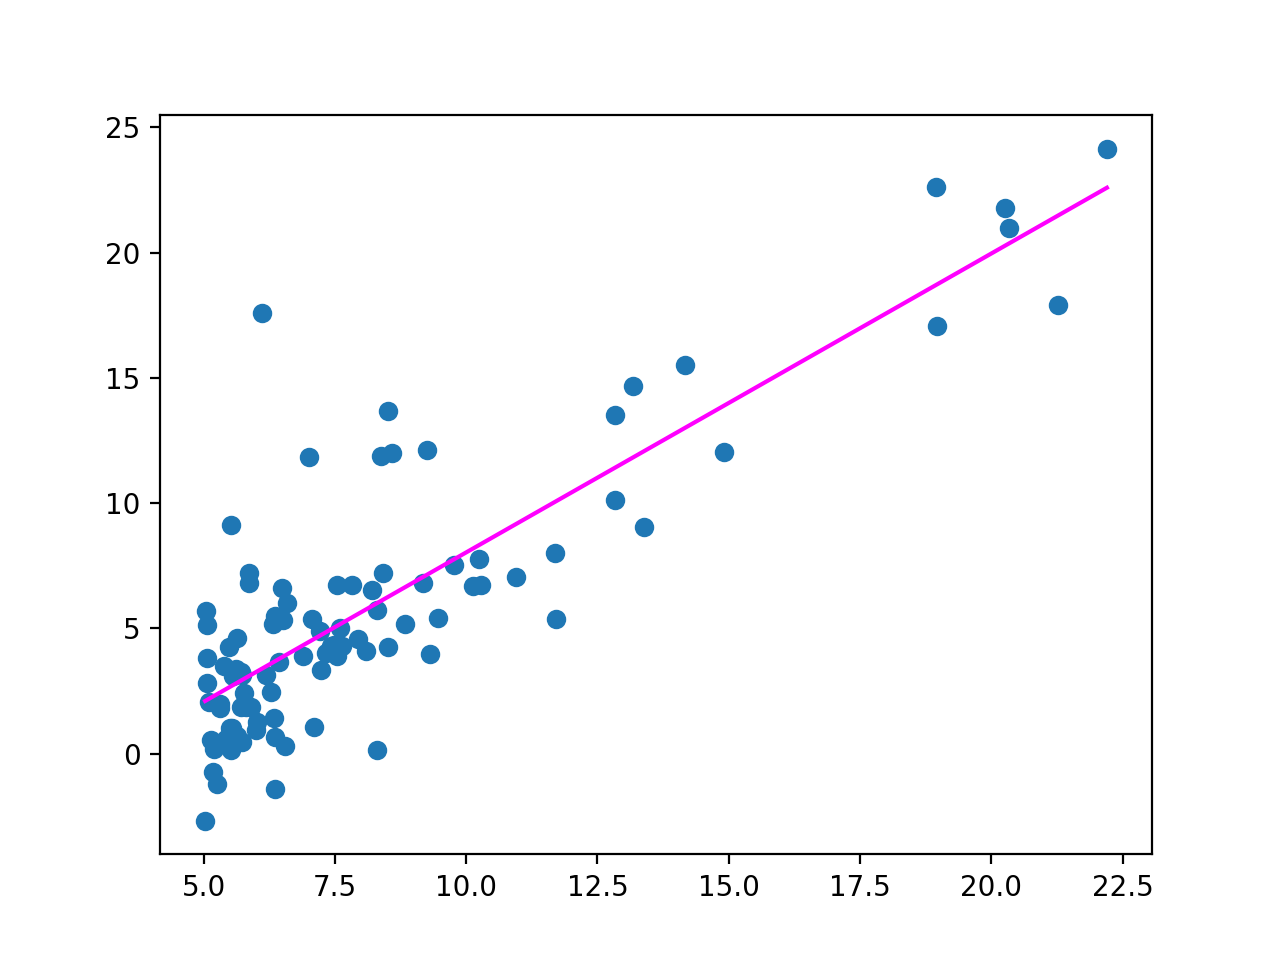
\includegraphics[width=\linewidth]{figs/Chap_1_Figure_2.png}
    \end{minipage}
    \vspace{-2ex}
\end{figure}

图中的洋红色直线即为梯度下降法得到的线性回归模型。

前文已经指出，学习率过大会导致迭代无法收敛，即 $J(\theta_0,\theta_1)$ 可能随迭代次数增加而增大。为了比较不同学习率对收敛过程的影响，可以绘制代价函数随迭代次数变化的曲线：

\begin{figure}[H]
    \centering
    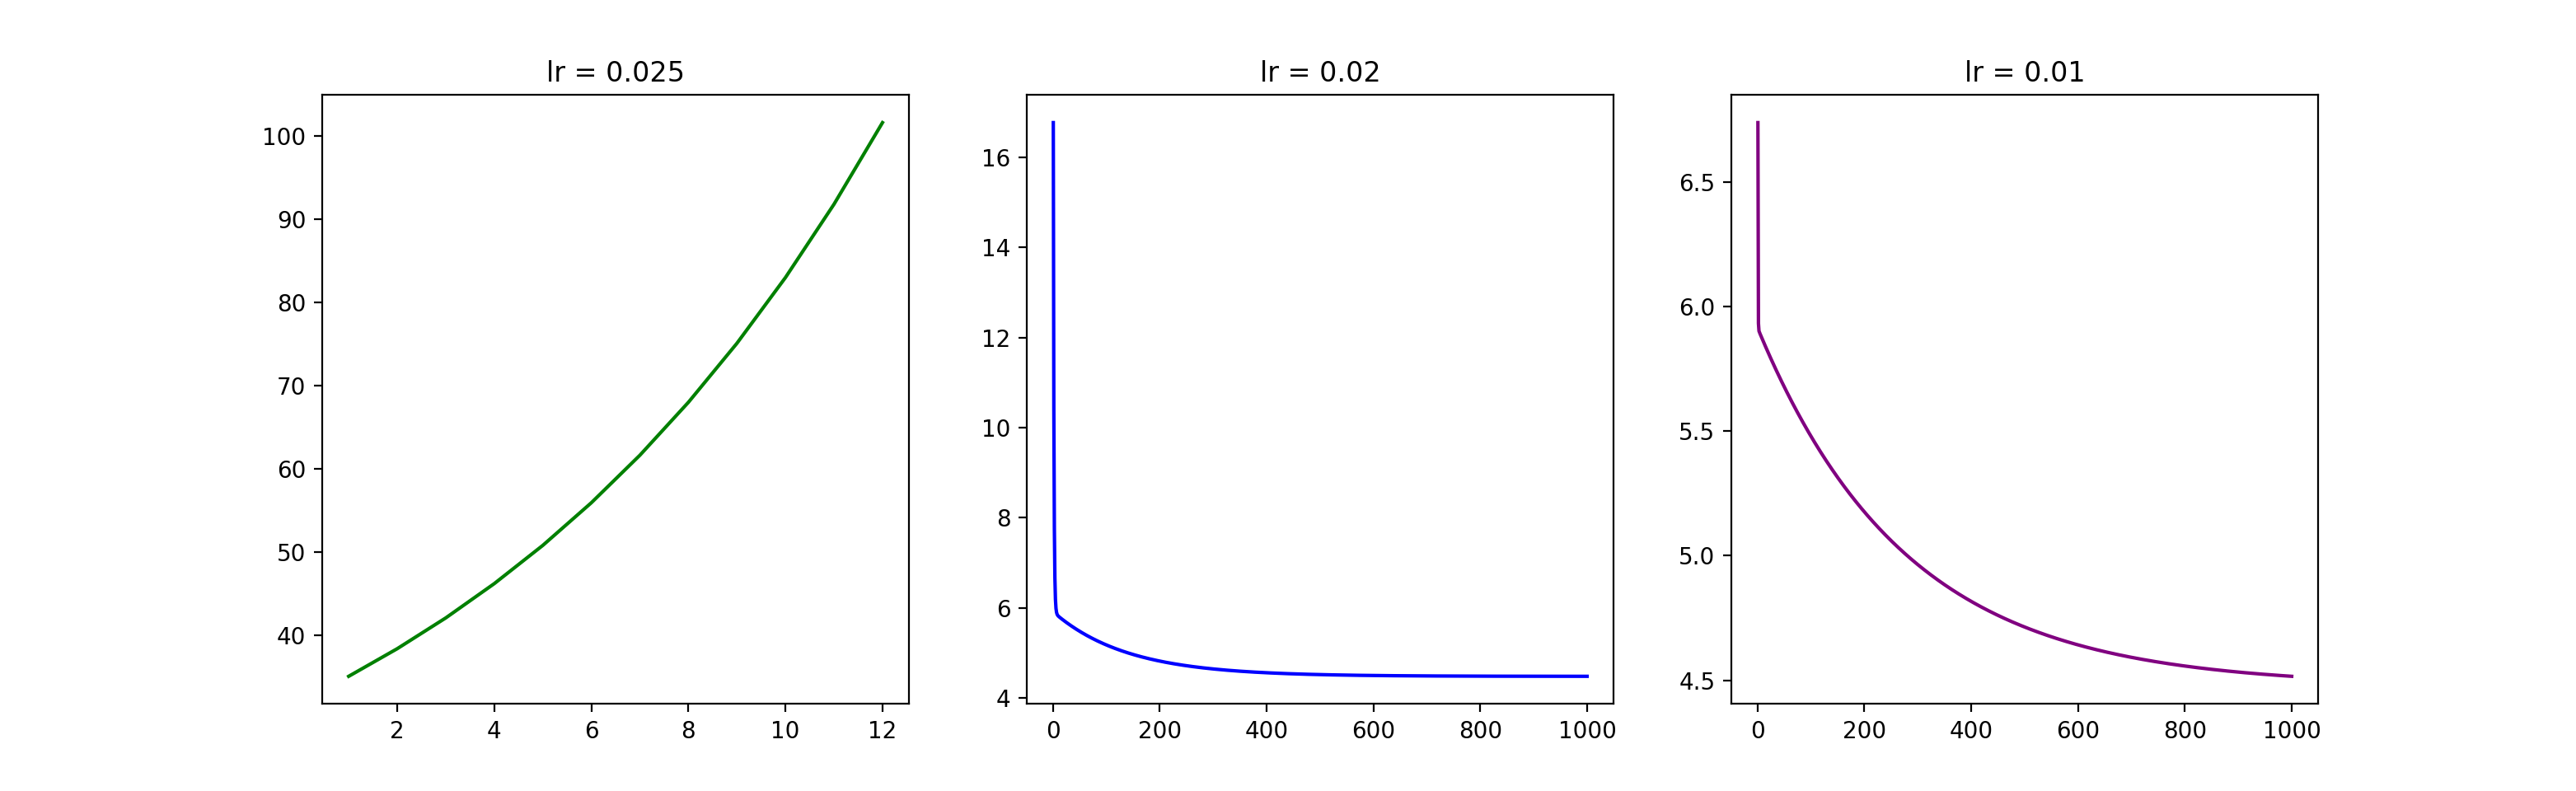
\includegraphics[width=\linewidth]{figs/Chap_1_Figure_3.png}
    \vspace{-3ex}
\end{figure}

由图可见，当学习率为 $0.025$ 时，代价函数呈发散趋势；当学习率分别为 $0.02$ 和 $0.01$ 时，代价函数能够逐步收敛。这一结果说明，学习率需要结合具体问题进行选择，适当的取值才能兼顾收敛速度与迭代稳定性。
